\section{Matching Key Points of Finger Nail Blood Vessel by Using VeriFinger}
\subsection{Detected Key Points Number}

On the last weekly report, I set the confidence threshold to 0.1 and the IOU threshold to 0.4, used leave-one-out protocol to get the matching scores for drawing ROC curve. From last week result, we can get that the performance from only ending points is better than only bifurcation. When we normalize the angle range, the matching performance of only bifurcation can be improved, but for matching with only-ending or with both ending and bifurcation, the corresponding matching performance is degraded. The last thing is that the performance will drop by normalize the image size to $384\times216$.

Firstly, I have calculated the number of ending, bifurcation, and dot points on the ground truth text files, as shown on the below Table \ref{ground-truth}. The total number is the total number of all 75 images (training set).

\begin{table}[h]
    \centering
    \caption{The number of key points on the ground truth}
    \begin{tabular}{ccccc}
    \hline
    Class       & Total (75 Images) & Min for Each Image & Max for Each Image & Average for Each Image \\ \hline
    Ending      & 21079             & 68                 & 550                & 281.053               \\
    Bifurcation & 5360              & 9                  & 358                & 71.467                 \\
    Dot         & 511               & 0                  & 34                 & 6.083                  \\ \hline
    \end{tabular}
    \label{ground-truth}
\end{table}

As for our detector, confidence threshold and IOU threshold will have effects on the number of detected key points. The main reason is that post-preprocessing of bounding box will use both of them to delete redundant bounding boxes. We can clearly get the difference from the Fig. \ref{detector-part}, at the same time, we can get the specific number of detected key points under different IOU and Confidence threshold from Table \ref{iou-conf}. 

\begin{figure}[h]
    \centering
    \subfloat[]{
    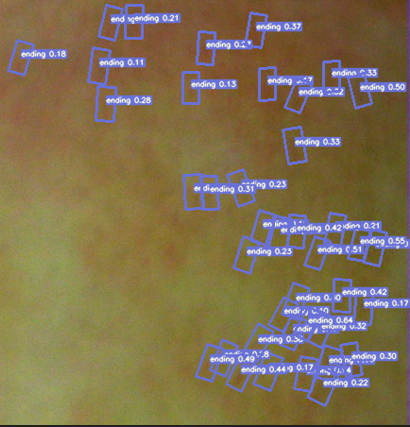
\includegraphics[width=1.63in]{Figure/02-09-2022/iou0.2-conf0.1.png}
    \label{iou0.2-conf0.1}}
    \subfloat[]{
    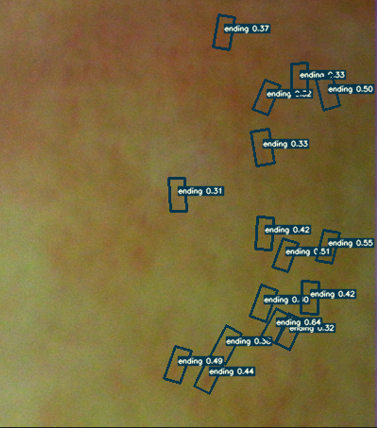
\includegraphics[width=1.5in]{Figure/02-09-2022/iou0.2-conf0.3.png}
    \label{iou0.2-conf0.3}}
    \subfloat[]{
    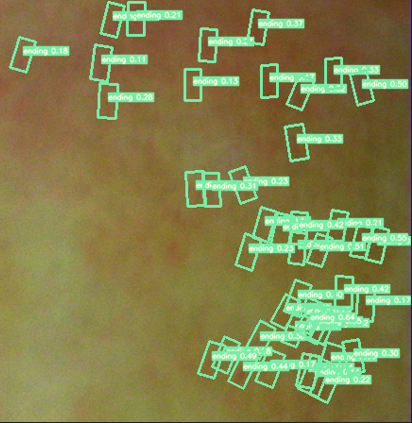
\includegraphics[width=1.65in]{Figure/02-09-2022/iou0.4-conf0.1.png}
    \label{iou0.4-conf0.1}}
    \subfloat[]{
    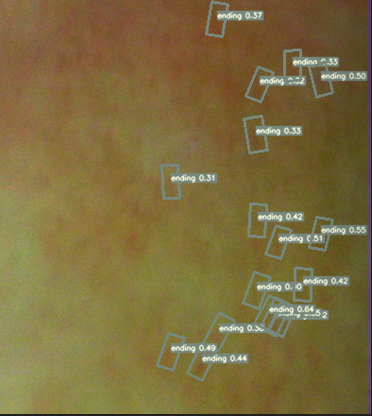
\includegraphics[width=1.52in]{Figure/02-09-2022/iou0.4-conf0.3.png}
    \label{iou0.4-conf0.3}}
    \caption{Small part of same image for showing difference of key point detection under different IOU and Confidence threshold. (a) IOU0.2-Conf0.1; (b) IOU0.2-Conf0.3; (c) IOU0.4-Conf0.1; (c) IOU0.4-Conf0.3.}
    \label{detector-part}
\end{figure}

% Please add the following required packages to your document preamble:
% \usepackage{multirow}
\begin{table}[h]
    \centering
    \caption{Number of Key Points on different IOU and confidence threshold}
    \begin{tabular}{ccccccc}
    \hline
    IOU                  & Confidence           & Class       & Total (75 Images) & Min for Each Image & Max for Each Image & Average for Each Image \\ \hline
    \multirow{2}{*}{0.2} & \multirow{2}{*}{0.1} & Ending      & 28919             & 110                & 500                & 385.587                \\
                         &                      & Bifurcation & 4386              & 8                 & 170                & 58.48                 \\ \hline
    \multirow{2}{*}{0.4} & \multirow{2}{*}{0.1} & Ending      & 30033             & 116                 & 500                & 400.44                \\
                         &                      & Bifurcation & 4879              & 8                  & 207                & 65.053                  \\ \hline
    \multirow{2}{*}{0.2} & \multirow{2}{*}{0.3} & Ending      & 20370             & 59                & 475                & 271.6                 \\
                         &                      & Bifurcation & 1606              & 0                 & 66                & 21.413                 \\ \hline
    \multirow{2}{*}{0.4} & \multirow{2}{*}{0.3} & Ending      & 21328             & 60                 & 499                & 284.373                \\
                         &                      & Bifurcation & 1642              & 0                  & 66                & 21.893                   \\ \hline
    \end{tabular}
    \label{iou-conf}
\end{table}


\subsection{Matching Performance}
We can use some threshold to change the output detected key points, as shown on Table \ref{iou-conf}. For approving matching performance under different IOU threshold and Confidence threshold, we use the same method to choose the ending points and bifurcations as shown on the Table \ref{number-of-key-points}. If the number of each type of key points on detected text files is larger than selected method, we will firstly delete low quality key points. On the contrary, we will keep all the detected key points. As shown on Fig. \ref{matching-performance}, although we use same selected method under different threshold, their performance still same not only on the leave-one-out protocol but also on the all-to-all protocol. From these results, we can easily get that the IOU and Confidence threshold can affect the number of detected key points. But it just has huge effects on the low quality key points. During our selected method, we will discard these low quality key points because number of key points already beyond 255. Therefor, these preserved key points are similar to each others.

\begin{table}[h]
    \centering
    \caption{}
    \begin{tabular}{ccccccc}
    \hline
    Key Point   & NO. & NO. & NO. & NO. & NO. & NO. \\ \hline
    Ending      & 255 & 128 & 64  & 193 & 96  & 48  \\
    Bifurcation & 0   & 0   & 0   & 62  & 32  & 15  \\ \hline
    \end{tabular}
    \label{number-of-key-points}
\end{table}

\begin{figure}[h!]
    \centering
    \subfloat[]{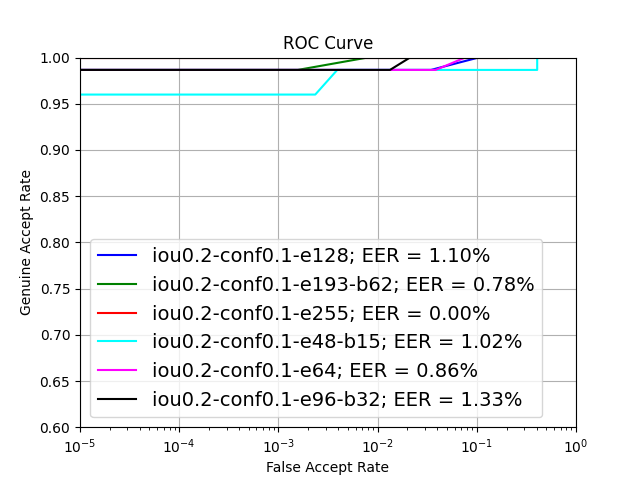
\includegraphics[width=1.74in]{Figure/02-09-2022/iou0.2-conf0.1-leave-one-out.png}%
    \label{iou0.2-conf0.1-leave-one-out}}
    \subfloat[]{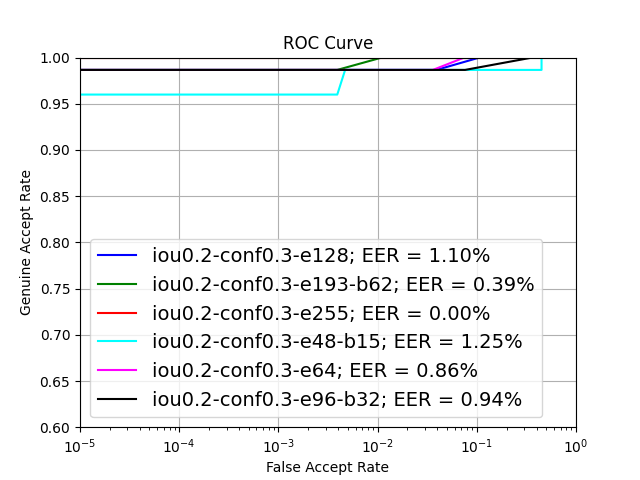
\includegraphics[width=1.74in]{Figure/02-09-2022/iou0.2-conf0.3-leave-one-out.png}%
    \label{iou0.2-conf0.3-leave-one-out}}
    \subfloat[]{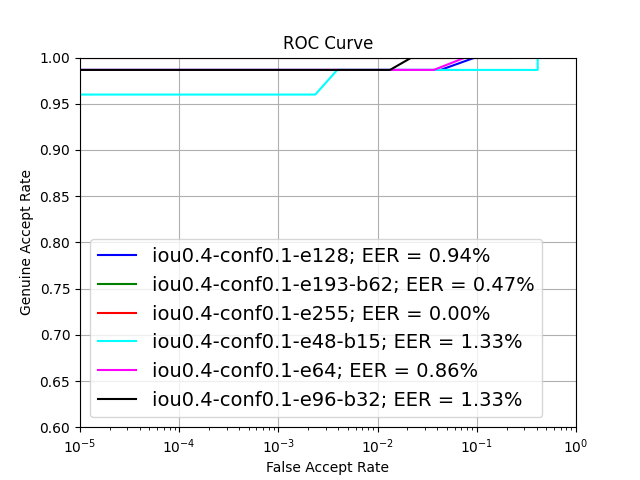
\includegraphics[width=1.74in]{Figure/02-09-2022/iou0.4-conf0.1-leave-one-out.png}%
    \label{iou0.4-conf0.1-leave-one-out4}}
    \subfloat[]{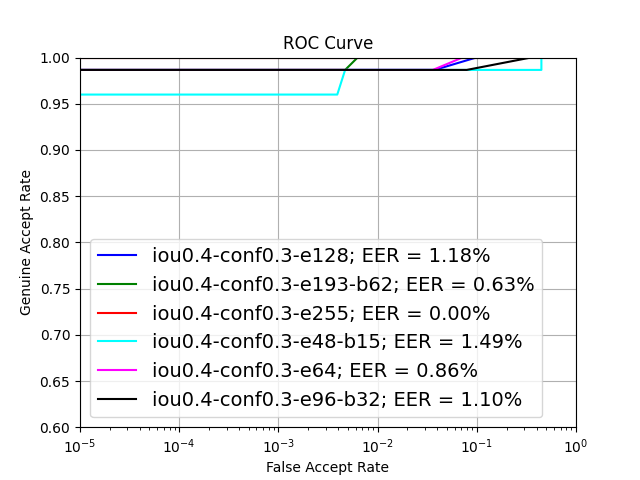
\includegraphics[width=1.74in]{Figure/02-09-2022/iou0.4-conf0.3-leave-one-out.png}%
    \label{iou0.4-conf0.3-leave-one-out}}

    \subfloat[]{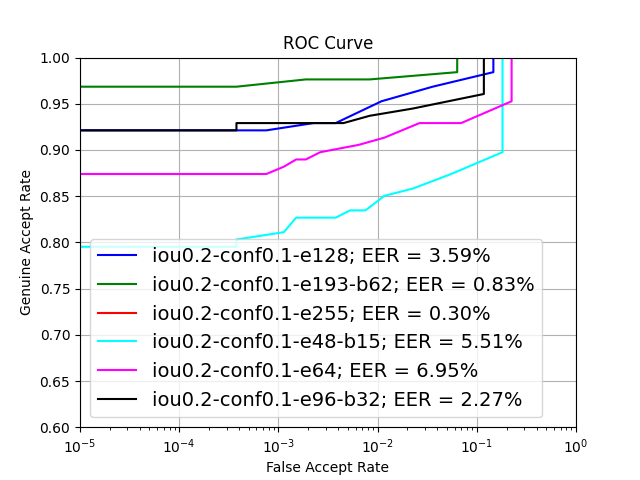
\includegraphics[width=1.74in]{Figure/02-09-2022/iou0.2-conf0.1-all-to-all.png}%
    \label{iou0.2-conf0.1-all-to-all}}
    \subfloat[]{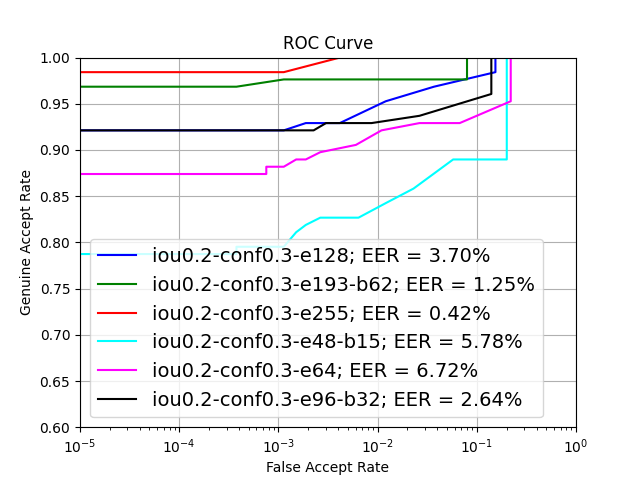
\includegraphics[width=1.74in]{Figure/02-09-2022/iou0.2-conf0.3-all-to-all.png}%
    \label{iou0.2-conf0.3-all-to-all}}
    \subfloat[]{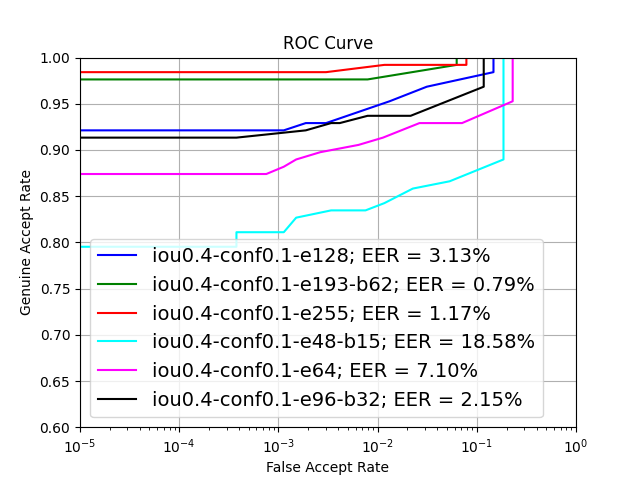
\includegraphics[width=1.74in]{Figure/02-09-2022/iou0.4-conf0.1-all-to-all.png}%
    \label{iou0.4-conf0.1-all-to-all}}
    \subfloat[]{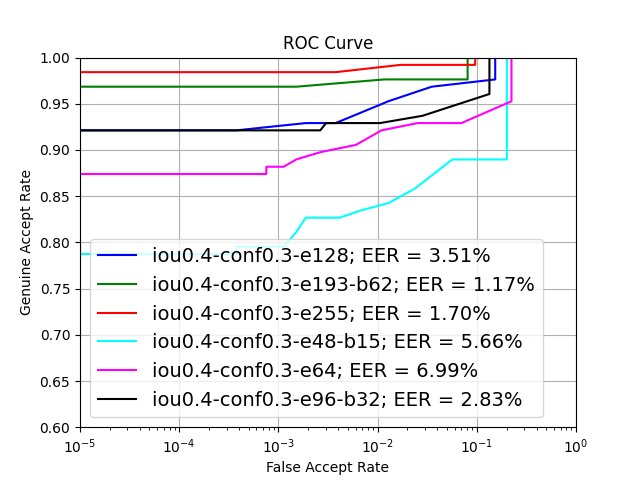
\includegraphics[width=1.74in]{Figure/02-09-2022/iou0.4-conf0.3-all-to-all.png}%
    \label{iou0.4-conf0.3-all-to-all}}
    
    \caption{These ROC curves all use the same screening method (Table \ref{number-of-key-points}) to perform screening of key points after detection at different IOU and Confidence thresholds. The top row uses the leave-one-out protocol and the bottom row uses the all-to-all protocol.}
    \label{matching-performance}
\end{figure}



\section{VR/AR Iris Recognition}
\subsection{Data Preprocessing}
Following the step of Eddie's paper, the preprocessing steps contain quality checker by using MobileNetV3, Iris detection by using SoloV2, and segmentation and normalization by using arc-support ellipse detector.
\subsubsection{Quality Detector}
The quality score is the probability predicted by MobileNet-V3, and predict the image belongs to which categories (good, bad, ugly). Depend on the quality score, author will discard bad and ugly Iris images for only keeping good Iris images. I follow the same method of Eddie's paper, but the number of preserved good Iris images is different with Eddie's paper, as the Table \ref{qulity-checker}. However the difference is small, only 7 images in total.

\begin{table}[h]
    \centering
    \caption{}
    \begin{tabular}{ccccc}
    \hline
                      & \multicolumn{2}{c}{Session1} & \multicolumn{2}{c}{Session2} \\ \hline
                      & L             & R            & L             & R            \\ \hline
    Number of Samples & 69120         & 69120        & 20070         & 20070        \\
    Good (Paper)      & 52563         & 53393        & 18107         & 17942        \\
    Good (Reproduce)  & 52560         & 53390        & 18106         & 17942        \\ \hline
    \end{tabular}
    \label{qulity-checker}
\end{table}

\subsubsection{Iris Detector}
Eddie used the SoloV2 as the backbone to detect and segment iris, pupil, sclera and eye. During this step, the SoloV2 model is too slow for instance segmentation. I have run the model for 48 hours, but it only processed half of the iris images.

\begin{figure}[h]
    \centering
    \subfloat[]{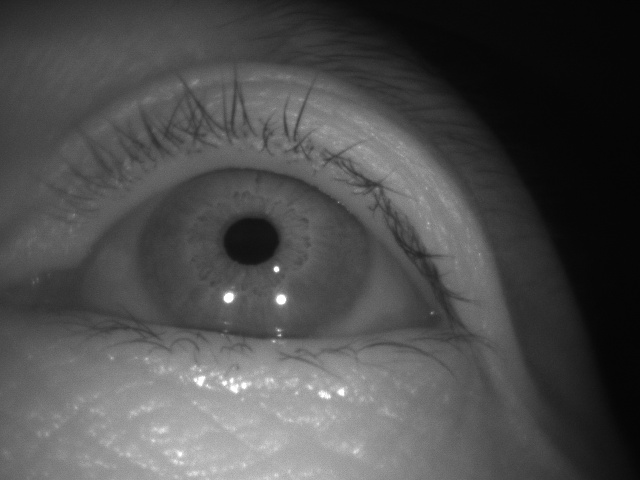
\includegraphics[width=1.74in]{Figure/02-09-2022/source_image.jpg}%
    \label{source_image}}
    \subfloat[]{
\includegraphics[width=1.74in]{Figure/02-09-2022/iris.jpg}%
    \label{iris}}
    \subfloat[]{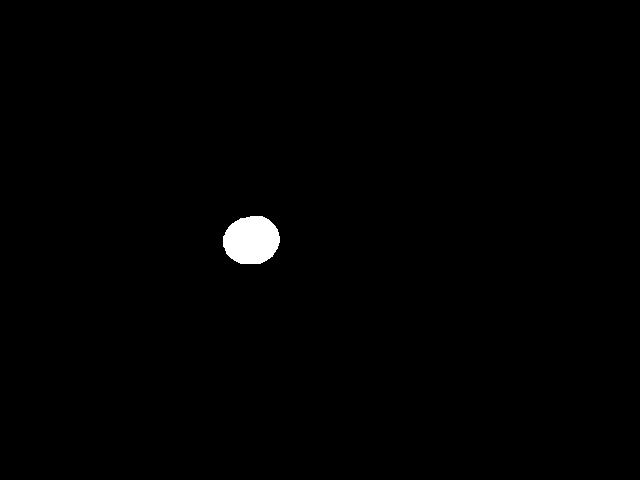
\includegraphics[width=1.74in]{Figure/02-09-2022/pupil.jpg}%
    \label{pupil}}
    \subfloat[]{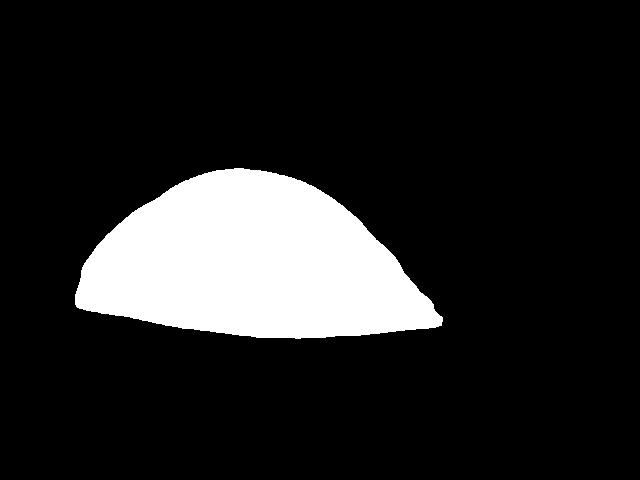
\includegraphics[width=1.74in]{Figure/02-09-2022/sclera.jpg}%
    \label{sclera}}

    
    \caption{Show segmentation result of one iris iamge sample.}
    \label{solov2-detector}
\end{figure}


\subsubsection{Iris Segmentation and Normalization}


\subsection{Recognition}
\subsubsection{Iris Recognition}
\subsubsection{Periocular Recognition}
\subsubsection{Adaptive Fusion}


